% AASTeX v6.2
%\documentclass[preprint]{aastex62}

% ApJ Format
\documentclass[iop,revtex4,twocolumn,apj,numberedappendix,appendixfloats]{emulateapj}
\usepackage{apjfonts}
% Hyperlinks & Bookmarks
\usepackage[pagebackref=false,colorlinks=true,citecolor=blue,linkcolor=blue,breaklinks=true,bookmarks=true]{hyperref}
\usepackage{amsmath}
\usepackage{comment}

% Units
\newcommand{\kms}{km~s$^{-1}$}
\newcommand{\msun}{$M_{\odot}$}
\newcommand{\msunyr}{$M_{\odot}~{\rm yr}^{-1}$}
\newcommand{\lsun}{$L_{\odot}$}
\newcommand{\ergs}{erg~s$^{-1}$}
\newcommand{\cmsq}{cm$^{-2}$}
\newcommand{\um}{$\mu$m}
\newcommand{\uJy}{$\mu$Jy}
\newcommand{\sqdeg}{deg$^2$}
\newcommand{\lx}{$L_{\rm X}$}
\newcommand{\lmir}{$L_{\rm 12\mu m}$}
\newcommand{\loiii}{$L_{\rm [OIII]}$}
% Emission lines
\newcommand{\Ha}{H$\alpha$}
\newcommand{\Hb}{H$\beta$}
\newcommand{\OII}{[O\,{\sc ii}]}
\newcommand{\OIIlam}{[O\,{\sc ii}]\,$\lambda$3727}
\newcommand{\SII}{[S\,{\sc ii}]}
\newcommand{\OIII}{[O\,{\sc iii}]}
\newcommand{\OIIIlam}{[O\,{\sc iii}]\,$\lambda$5007}
\newcommand{\NII}{[N\,{\sc ii}]}
\newcommand{\NeIII}{[Ne\,{\sc iii}]}
% special 
\newcommand{\nod}{\nodata}

\newcommand{\angstrom}{\mbox{\normalfont\AA}}
\newcommand{\reff}{$R_{\rm eff}$}
\newcommand{\ewha}{EW(H$\alpha$)}
\newcommand{\logm}{log($M/M_{\odot}$)}
%\newcommand{\arcsec}{\prime\prime}
\newcommand{\simard}{Simard+11}

% citations
\defcitealias{Fu:2018}{Paper I} 

\usepackage{epstopdf}

\begin{document}

\title{
SDSS-IV MaNGA: The Radial Profile of Enhanced Star Formation in Close Galaxy Pairs
}

\author{
Joshua~L.~Steffen\altaffilmark{1}, Hai~Fu\altaffilmark{1,2}, J.~M.~Comerford\altaffilmark{3}, Y.~Sophia~Dai\altaffilmark{4}, Shuai~Feng\altaffilmark{5,6,7}, Arran~C.~Gross\altaffilmark{1}, and Rui~Xue\altaffilmark{1}
}
\altaffiltext{1}{Department of Physics \& Astronomy, University of Iowa, Iowa City, IA 52242}
\altaffiltext{2}{Insititute for Astronomy, University of Hawaii, Honolulu, HI 96822}
\altaffiltext{3}{Department of Astrophysical and Planetary Sciences, University of Colorado, Boulder, CO 80309}
\altaffiltext{4}{Chinese Academy of Sciences South America Center for Astronomy (CASSACA), 20A Datun Road, Beijing 100012, China}
\altaffiltext{5}{Department of Physics, Hebei Normal University, 20 South Erhuan Road, Shijiazhuang, 050024, China}
\altaffiltext{6}{Key Laboratory for Research in Galaxies and Cosmology, Shanghai Astronomical Observatory, Chinese Academy of Sciences, 80 Nandan Road, Shanghai 200030, China}
\altaffiltext{7}{University of the Chinese Academy of Sciences, No.19A Yuquan Road, Beijing 100049, China}


\begin{abstract}
We compare the radial profiles of the specific star formation rate (sSFR) in a sample of 175 star-forming galaxies in close pairs with those of mass-matched isolated galaxies in the SDSS-IV MaNGA survey. We find that the sSFR is centrally enhanced (within one effective radius) in interacting galaxies by $\sim$0.25 dex and that there is a weak sSFR suppression in the outskirts of the galaxies of $\sim$0.1 dex. We stack the differences profiles for galaxies in five stellar mass bins between \logm\ $=$ 9.0$-$11.5 and find that the sSFR enhancement has no dependence on the stellar mass. The same result is obtained when the comparison galaxies are matched to each paired galaxy in both stellar mass and redshift. In addition, we find that that the sSFR enhancement is elevated in pairs with nearly equal masses and closer projected separations, in agreement with previous work based on single-fiber spectroscopy. We also find that the sSFR offsets in the outskirts of the paired galaxies are dependent on whether the galaxy is the more massive or less massive companion in the pair. The more massive companion experiences zero to a positive sSFR enhancement while the less massive companion experiences sSFR suppression in their outskirts.
\end{abstract}

\keywords{galaxies: star formation --- galaxies: nuclei --- galaxies: interactions --- galaxies: mass evolution}

%%%%%%%%%%%%%%%%%%%%%%%%%%%%%%%%%%%%%%%%%%%%%%%%%%%%
\section{Introduction}\label{sec:intro}

%%%Galaxy Evolution%%%
In the $\Lambda$CDM model, galaxy evolution is a hierarchical process. In this model, massive galaxies are the product of several past merger events of smaller galaxies. In fact, cosmological hydrodynamical simulations have shown that repeated merger events may be responsible for as much as $\sim$60\% of stellar mass in massive galaxies like M87 \citep[e.g.,][]{Rodriguez-Gomez:2016,Pillepich:2018}. As the galaxies undergo the merging process, the gas within the galaxies are subject to gravitational torques which perturb the morphology of the galaxies.

%%%Simulations%%%
The internal dynamics of these interacting galaxies were first modeled in the seminal work, \citet{Toomre:1972}. Since then, hydrodynamical simulations have expanded upon the N-body simulations of \citet{Toomre:1972} by modeling gas-dynamics within the galaxies. These simulations show how barred structures develop within the disks of the interacting galaxies due to the tidal torques between them \citep{Barnes:1991}. As the bars form, the gases within the galaxy's disk lose angular momentum and get funneled into the centers of the galaxies. 

When the gas-inflows impact upon the gases in the nucleus of galaxy a burst of new star formation in triggered \citep{Barnes:1996, Mihos:1996}. These gas inflows will also bring metal-poor gases from the disk into the center of the galaxy which can dilute the central metallicity \citep{Rupke:2010, Perez:2011, Scudder:2012}. The gas-inflows may also be able to reach the very center of the galaxy and trigger supermassive black hole (SMBH) accretion \citep{Capelo:2017}. 

%%%Observations%%%
Interaction induced star formation was first seen observationally in the bluer colors of peculiar galaxies in \citet{Larson:1978}. This observation has also been shown in more recent works using the single-fiber spectroscopic survey, SDSS (Sloan Digital Sky Survey) \citep{Ellison:2008, Li:2008, Scudder:2012, Patton:2013, Bustamante:2020}. From these previous works it has been shown that the strength of the star formation enhancement in the centers of paired galaxies is dependent on the stellar mass of the pairs \citep{Li:2008}, the projected separation between the pairs \citep{Ellison:2008, Li:2008, Scudder:2012}, and the mass ratio between the pairs \citep{Ellison:2008}. 

%%%Integral Field Spectroscopy%%%
The previous mentioned works using SDSS were restricted to studying the centers of the paired galaxies through 2\arcsec\ diameter optical fibers. With the recent large integral field spectroscopic (IFS) surveys, interacting galaxies can now be studied with unprecedented spatial detail. These surveys allow us to study the centers of merging galaxies more rigorously since apertures can be set to the physical scale of the galaxies instead of being bound by a fixed sky aperture. These IFS surveys will also allow us to see the extent of the centrally induced star formation and to see how the star formation in the disks of the galaxies are affected. 

Indeed, \citet{Barrera-Ballesteros:2015} used the CALIFA (Calar Alto Legacy Integral Field Area) survey to study a sample of 103 paired galaxies by varying the size of the aperture through which the \ewha\ is extracted from. In this study, they found a moderate enhancement to the sSFR in the centers of paired galaxies and a moderate suppression to the sSFR in outskirts of the paired galaxies. 
%
\citet{Pan:2019} used the SDSS-IV MaNGA survey to study radial profiles of a sample of 205 paired galaxies. The enhancement to the sSFR was shown to be the strongest in the centers of the paired galaxies. This central enhancement linearly fell with increasing galactocentric radii; however, a moderate enhancement to the sSFR remain in the outskirts of the galaxies. \citet{Pan:2019} further studied the paired galaxies as a function of merger stage; from well separated pairs to post-merger galaxies. Across the different merger stages, the sSFR enhancement was greatest in close pairs with tidal features and in post-merger galaxies. This was in agreement with previous hydrodynamical simulations which showed that a burst of star formation is triggered after the first pericenter and as the two galaxies begin to coalesce \citep{Scudder:2012}. 
%
The radial profile of sSFR in post-merger galaxies has also been studied with the MaNGA survey by \citet{Thorp:2019}. The post-merger galaxies were shown to have a strong enhancement to the sSFR in their centers as well as a moderate enhancement in their outskirts. 

Where previous studies on the radial profile of the sSFR offsets in paired galaxies have focused on studying the profiles as a function of interaction stage, we will focus on the radial profile as a function of the stellar mass, projected separation, and mass ratio. As mentioned previously, these parameters have been covered by studies restricted to the nuclear region of the paired galaxies. With the MaNGA survey, we will be able to expand upon these previous studies in greater spatial detail. We will be able to see how these three parameters affect both the level of the sSFR offsets in the centers of the paired galaxies and the offsets in the outskirts of the galaxies. We will also be able to study if any of three parameters influence the gradient of the sSFR enhancement profiles or if the gradient is preserved between different configurations. 

In our previous work using the MaNGA data included in the 14th Public Data Release \citep[DR14;][]{Abolfathi:2018}, we built a sample of close galaxy pairs where both components of the pair were contained within the field of view of a single integral field unit \citep[][hereafter \citetalias{Fu:2018}]{Fu:2018}. We found that approximately 5.7\% of the MaNGA galaxies have a companion galaxy contained within the field-of-view of a single IFU. In this work, we update this sample and supplement it with a sample of companion galaxies identified outside the field-of-view of the MaNGA IFUs. 

% Organization
This paper is organized as follows; in Section \ref{sec:data} we will discuss the properties of the MaNGA survey along with the construction of our pair and control samples, in Section \ref{sec:analysis} we will discuss how we measure star formation rates and how we build radial profiles of star formation, in Section \ref{sec:results} we study the radial profiles as a function of stellar mass, projected separation, and the mass ratio, in Section \ref{sec:disc} we compare our work against previous works, and in Section \ref{sec:sum} we summarize the findings of the work. 
% cosmology
Throughout we adopt the $\Lambda$CDM cosmology with $\Omega_{\rm m}=0.3$, $\Omega_\Lambda=0.7$, and $h=0.7$. 

%%%%%%%%%%%%%%%%%%%%%%%%%%%%%%%%%%%%%%%%%%%%%%%%%%%%
\section{Data and Samples}\label{sec:data}

%%%%%%%%%%%%%%%%%%%%%%%%%%%%%%%%%%%%%%%%%%%%%%
\begin{figure}
\centering
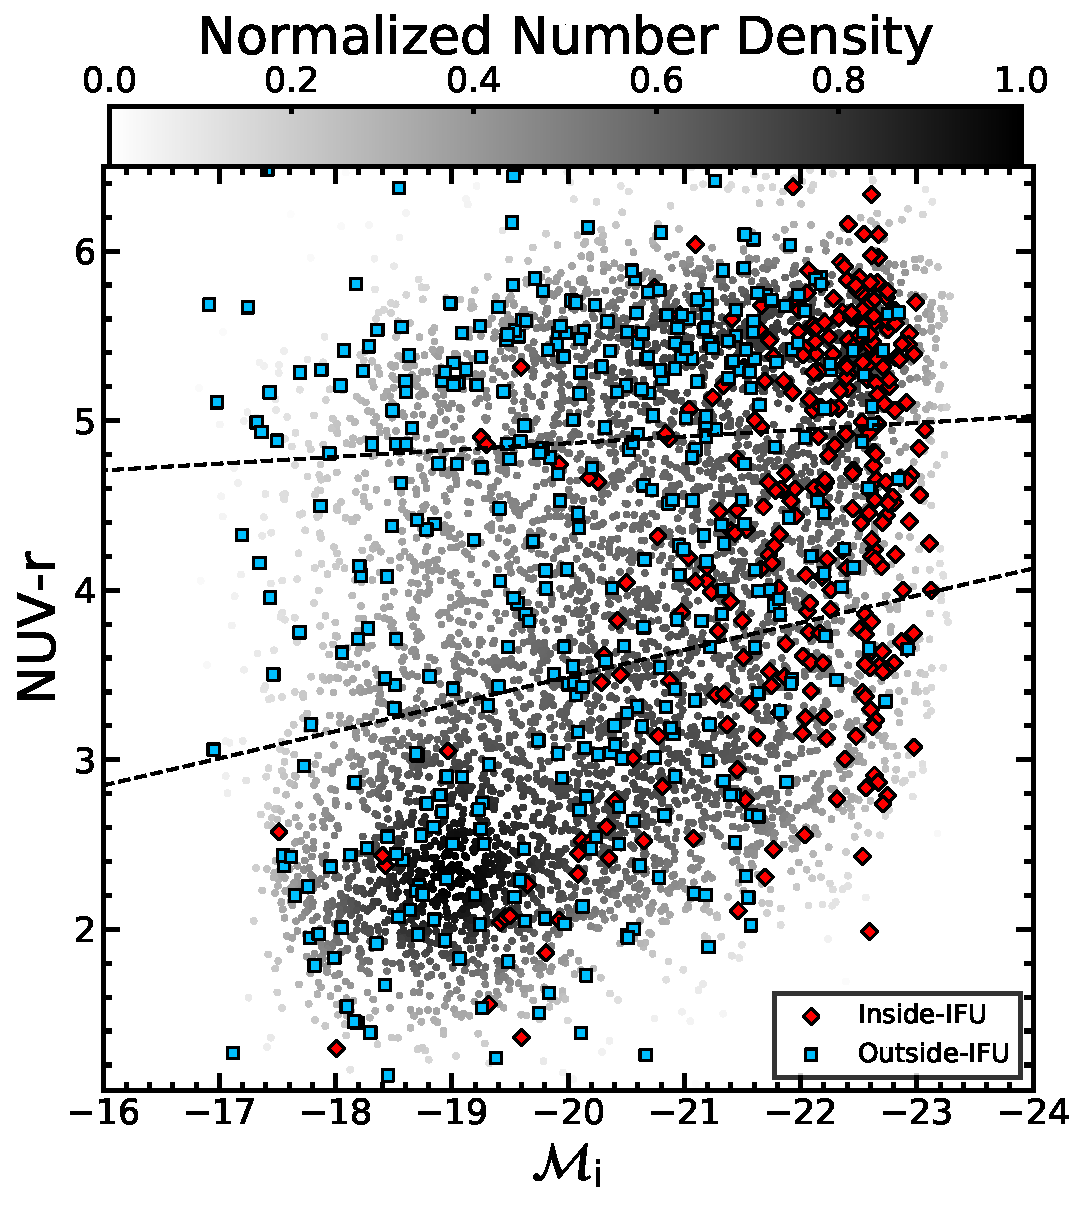
\includegraphics[width=\linewidth]{fig/color-mag.pdf}
\caption[]{Color-magnitude diagram for MaNGA galaxies. The grey circles represent the whole MaNGA sample and reflects the local density around each data point in this color-magnitude plane, as indicated by the color bar on the top. Inside-IFU pairs are marked with red diamonds and the outside-IFU pairs are marked with red squares. From top to bottom, the dashed lines divide the sample into red sequence, green valley, and blue cloud. The star-forming galaxy sample used in this paper are the galaxies below the lower dividing line.}
\label{fig:cmd}
\end{figure}
%%%%%%%%%%%%%%%%%%%%%%%%%%%%%%%%%%%%%%%%%%%%%%

MaNGA is an IFS survey at the Apache Point Observatory (APO) which used the SDSS (Sloan Digital Sky Survey) 2.5-meter telescope along with two dual-channel BOSS spectrographs \citep{Drory:2015}. MaNGA captures spectra through 17 integral field units (IFUs) with variable numbers of fibers; 19, 37, 61, 91, and 127 fibers covering 12.5\arcsec, 17.5\arcsec, 22.5\arcsec, 27.5\arcsec, and 32.5\arcsec on the sky respectively \citep{Law:2015}. MaNGA is an optical survey with a spectral coverage of 3600$-$10,300 \AA\ with a resolution of R $\sim$ 2000 and a PSF of 2.5\arcsec\ FWHM \citep{Bundy:2015}. 

The MaNGA survey targets galaxies from a subset of 41,154 galaxies in the NASA-Sloan Atlas (NSA v1\_0\_1; \url{http://www.nsatlas.org}) with a redshift range of 0.01 $< z <$ 0.15 and a luminosity range of -17.7 $<$ $\mathcal{M_i}$ $<$ -24.0, where $\mathcal{M_i}$ is the rest frame $i$-band magnitude within the survey's elliptical Petrosian apertures. MaNGA plans to cover 10,000 galaxies with a flat stellar mass distribution at two spatial coverages, 1.5 \reff\ and 2.5 \reff\ (where \reff\ is the radius which contains 50\% of the galaxy's total light). In this work we use the data from the 8th MaNGA Product Launch (MPL-8), which covers 6142 unique galaxies observed by July 3, 2018. 

We classify galaxies in this survey as star forming galaxies by selecting galaxies in the blue cloud on the color-magnitude diagram (CMD). We show the CMD for the MaNGA survey and our pair sample in Figure \ref{fig:cmd} along with demarcation lines which separate the blue cloud, red sequence, and green valley. We established the demarcation lines by collapsing the CMD to a color histogram for each of the three regions. We then varied the slopes between the regions until we found the slopes which best fit the data. These demarcation lines are;

\begin{equation}\label{eq:blue}
NUV-r = 3.1682 - 0.16 (\mathcal{M}_i+18)
\end{equation}
\begin{equation}\label{eq:red}
NUV-r = 4.7866 - 0.04 (\mathcal{M}_i+18)
\end{equation}

Where $NUV-r$ is the color from SDSS's $k$-corrected absolute magnitude and $\mathcal{M}_i$ is the $i$-band magnitude from the NSA catalog. We further apply an \ewha\ $\ge$ 3\AA\ cut on galaxy spectra extracted from a 1.0~\reff\ aperture to ensure that all passive galaxies are removed from the sample \citep{Cid-Fernandes:2011}. Finally, we use the BPT diagnostic \citep{Baldwin:1981} to remove galaxies with possible AGN in their centers. Specifically, we use the emission line ratios, log([O~{\sc iii}]/H$\beta$) and log([N~{\sc ii}]/H$\alpha$), extracted from a 1.3~kpc aperture along with the maximum starburst line of \citet{Kewley:2001} as the demarcation between the star-forming branch and the AGN branch.

On top of the star formation cuts, we require that all galaxies are in either the Primary or Secondary MaNGA subsamples \citep{Wake:2017}, and that the stellar mass range of the galaxy sample is between \logm\ $=$ 9.0$-$11.5. We use masses calculated from the elliptical Petrosian apertures in the NSA catalog for our total stellar masses. 

We build two different pair samples in this work; the inside-IFU sample which contains paired galaxies where both galaxies are covered by a single MaNGA IFU and the outside-IFU sample where a MaNGA target galaxy is coupled with another galaxy found outside of its MaNGA IFU. 

\subsection{Inside-IFU Sample}\label{sec:inside}

We identify potential paired galaxies by overlaying SDSS photometric objects over the MaNGA fields of view. We manually inspect each MaNGA field, removing photometric objects which are over-deblended galaxy fragments and adding any objects missed by the SDSS photometric catalog. At this stage the object catalog includes any foreground stars and foreground/background galaxies along with the potential paired galaxies. 

To select paired galaxies out of our object catalog, we inspect the spectra of each object. We use our own {\sc idl} based spectral fitting code, {\sc spfit}, to model the spectra from the MaNGA datacubes. {\sc spfit} simultaneously fits emission lines and the stellar continuum with the Levenberg-Marquardt nonlinear least-squares minimization algorithm \citepalias{Fu:2018}. Emission lines are parameterized as a Gauss-Hermite series and the stellar continuum is the sum of simple stellar populations (SSPs) convolved with the line-of-sight velocity distribution (LOSVD).

The spectra of the identified objects is extracted through a 1\arcsec\ circular aperture and fitted assuming the MaNGA target's redshift and then manually sorted into the following categories; ``good" galaxy spectra, broad-line AGN, foreground star, foreground/background galaxies, or poor S/N objects. The ``good" galaxy spectra are the objects whose spectra are well modeled by {\sc spfit} at the target galaxy's redshift, whether it is the target galaxy itself or a nearby companion galaxy. This means that the companion galaxy can be within approximately $\pm$3000 km s$^{-1}$ of the MaNGA target. We found 6573 ``good" objects, 57 broad-line AGN, 836 foreground stars, 319 foreground/background galaxies, and 1546 objects with poor S/N. 

From the 6573 galaxies with good spectra, 404 of the MaNGA IFUs have multiple galaxy objects within the IFU. We further restrict the sample by setting a relative velocity cut of $\Delta v$ $<$ 500 km s$^{-1}$ to remove projected companions. Given redshift range of the MaNGA sample and the size of MaNGA's IFUs, the maximum projected separation for a companion galaxy in the IFU is $\sim$40 kpc. Again, the galaxy sample is also restricted to galaxies with a stellar mass range of \logm\ $=$ 9.0$-$11.5 and galaxies in the Primary or Secondary MaNGA subsamples. We also require that the galaxies are classified as star forming as described in Section \ref{sec:data}. These requirements reduce our sample down to 87 star forming galaxies (SFGs). 

Several of the target galaxies in our sample have multiple companions. From the whole set of 404 IFUs, there are 327 pairs, 67 triplets, 7 quadruplets, and 1 quintuplet. In cases where a MaNGA target has multiple viable companions galaxies, we chose the closest companion when measuring the pair's mass ratio and projected separation. 



\subsection{Outside-IFU Sample}\label{sec:outside}

We supplement the inside-IFU sample with a set of pairs identified outside of the field of view of the MaNGA IFU. We select these outside-IFU pairs from the NSA catalog. We search for these external pairs by selecting objects with a projected separation from the MaNGA targets of $r_{\rm p}$ $<$ 50 kpc using the MaNGA target's redshift. We further use a relative velocity cut of $\Delta v$ $<$ 500 km s$^{-1}$ to remove projected galaxies from the selection. 

From the NSA catalog's 641,409 galaxies, we find 492 galaxies which are paired to MaNGA targets. After restricting the sample to SFGs, we have 133 MaNGA targets with paired galaxies outside of the IFU. MaNGA targets which have both an inside-IFU and an outside-IFU pair are left to the inside-IFU sample. This give use a total of 175 MaNGA targets in our pair sample.

\subsection{Control Sample}\label{sec:control}

To show how the population of galaxy pairs differs from isolated galaxies, we will compare our pair sample to a sample of isolated galaxies in the MaNGA survey. We build this control sample from the MaNGA target galaxies which have no spectroscopic companions within $r_{\rm p}$ $<$ 50 kpc and $\Delta v$ $<$ 500 km s$^{-1}$ either inside or outside of the IFU. This gives us a control sample of 1888 star forming control galaxies. 

It has been shown that the SFR in galaxies is dependent on both the stellar mass and the redshift of the galaxies \citep{Noeske:2007}. We will compare our interacting galaxies with isolated galaxies of a similar stellar mass and redshift, to account for these other dependencies. To do this, we will use two different methods of pair - control comparison. 

In the first method, we only control for the stellar mass between the pairs and controls. We split both the pair and control samples into five evenly spaced stellar mass bins over the range, \logm\ $=$ 9.0$-$11.5. The pairs are then compared to their respective controls within each stellar mass bin. While the redshift in not constrained in this method, we will show in Section \ref{sec:mass-bin} that this method is sufficient to reveal the merger induced star formation. 


In the second method, we wish to account for both stellar mass and redshift. To do this we select a subsample of 20 control galaxies for each paired galaxy. We first select all of the control galaxies which are within a 0.1 dex stellar mass limit and within the same MaNGA subsample (e.g. Primary or Secondary) as the paired galaxy. Since the MaNGA sample has a tight distribution in stellar mass and redshift, the stellar mass and MaNGA subsample restriction effectively sets a $z$ $\lesssim$ $\sim$0.025 redshift cut. 

Setting the above requirements, most paired galaxies will find between 20$-$100 control galaxies. Since we want each paired galaxy to be treated in a similar manner, we will down-select the total number of acquired control galaxies down to 20 controls randomly. A given control galaxy may be selected for multiple pairs by the pipeline; most of the control galaxies are used at least once and the average number of times a given control is reused is between 4$-$6 times. In the cases where a paired galaxy does not initially acquire 20 control galaxies we iteratively expand the stellar mass limit by 0.1 dex until at least 20 control galaxies are found. Only 5 of the paired galaxies required an extra iteration to find 20 controls. 

%%%%%%%%%%%%%%%%%%%%%%%%%%%%%%%%%%%%%%%%%%%%%%%%%%%%
\section{Radial Profiles of Star Formation}\label{sec:analysis}

\subsection{Specific Star Formation Rate}

%%% SPFIT
We use our spectral fitting code, {\sc spfit}, to get measurements of emission line fluxes, equivalent widths, velocities, and velocity dispersions of 19 emission lines and measurements of stellar masses, ages, [Fe/H], and the kinematics of the stellar populations. 

%%% Reddening
We correct the emission lines for reddening using the extinction curve from \citet{Cardelli:1989} with updated coefficients from \citet{ODonnell:1994}. The extinction is parameterized as $R_V$ $\equiv$ $A_V/E(B-V)$ $=$ 3.1, where we estimate the value of the $V$-band extinction, $A_V$, by comparing the H$\alpha$/H$\beta$ ratio to the expected value of 2.85 for case-B recombination. 

We measure the SFR from the extinction corrected H$\alpha$ luminosity, $L_{{\rm H}\alpha}$.  We use the SFR formula, Equation \ref{eq:sfr}, from \citet{Murphy:2011} which uses a Kroupa IMF, Solar metallicity, a constant SFR at an age of 100 Myr, and Case-B recombination. 

\begin{equation}\label{eq:sfr}
\frac{\rm{SFR}}{M_{\odot} \, \rm{yr^{-1}}} = \frac{L_{\rm H\alpha}}{1.86 \times 10^{41}\, \rm{erg\,s}^{-1}}
\end{equation}

Since the stellar mass of a galaxy is not uniformly distributed within the galaxy, we normalize the SFR by the local stellar mass, $M$, giving us the specific star formation rate (sSFR). The local stellar masses used here is the stellar mass calculated by {\sc SPFIT}'s fit to the stellar continuum within each MaNGA spaxel (spatial pixel).

\begin{equation}
{\rm sSFR} = \frac{\rm SFR}{M}
\end{equation}

This will allow us to compare regions of high mass surface density to regions of low mass surface density. 

%%%%%%%%%%%%%%%%%%%%%%%%%%%%%%%%%%%%%%%%%%%%%%%%%%%%
\subsection{Radial Profiles}\label{sec:radial}

In order to spatially characterize the star formation in the paired galaxies we build radial profiles of sSFR. First, the geometry of the galaxies needs to be defined. Specifically we will need the position angle, the inclination angle, and the effective radius of each of the MaNGA targets. We use the $r$-band elliptical Petrosian apertures from the NSA catalog and the $r$-band S\'ersic apertures from \citet{Simard:2011} to define the geometries of the galaxies. 

The NSA catalog has complete coverage over the MaNGA sample (since MaNGA selects its targets from this catalog); however, it tends to fail to properly fit paired galaxies with close on-sky separations. We found that the apertures from \citet{Simard:2011} work better for these close paired galaxies; however, the catalog does not completely cover the MaNGA sample. We use the NSA catalog for the outside-IFU pair sample because they are well separated on the sky. The \citet{Simard:2011} catalog is used for the inside-IFU sample. If the paired galaxy is not covered by \citet{Simard:2011}, we use the ellipse from the NSA catalog. 

We fit the geometry with apertures from both catalogs when available. When using the first method of pair-control comparison, where pairs and controls are grouped into stellar mass bins, we fit the control galaxies with the NSA apertures. When making the comparison with the second tailored control method, paired galaxies fitted with the NSA aperture are compared against controls fitted with the NSA aperture and paired galaxies fitted with the \citet{Simard:2011} apertures are compared against controls fitted with the \citet{Simard:2011} apertures. Further, when defining the a galaxy's geometry with the \citet{Simard:2011} apertures we also use the masses given in the catalog for the total stellar mass of the galaxy.



We calculate the inclination angle, {\it i}, of the galaxies using the major-to-minor axis ratios from the elliptical apertures;

\begin{equation}
{\rm cos^2}(i) = \frac{(b/a)^2 - q^2}{1 - q^2}
\end{equation}

Where $b/a$ is the major-to-minor axis ratio and $q$ is the intrinsic oblateness. We use the empirically determined oblateness of $q = 0.13$, from \citet{Giovanelli:1994}.

The inclination angle, along with the galaxy's position angle, is used to deproject the geometries of the galaxies. We use the 50\% half light radius (i.e. the effective radius, \reff) to scale the sizes of the galaxies. Doing this will allow us to compare galaxies of different sizes against each other.

Once the geometry of the galaxies are set, we can build the radial profiles. The spaxels are binned into radius increments of 0.2 \reff\ from 0.0$-$2.6 \reff. Within each radius bin we take the median of the specific star formation rate. The profiles' errors are the standard error of the mean of the data within each radius bin. We create one of these individual averaged radial profiles for every MaNGA galaxy. 

%We use our catalog of photometric objects and the \citet{Simard:2011} catalog to mask foreground/background objects within the MaNGA IFUs which may contaminate the data. Objects in our photometric catalog are masked out with a 2\arcsec\ circular aperture and the galaxies from \citet{Simard:2011} are masked out with a 2.0 R/\reff\ elliptical aperture, using the r-band S\'ersic apertures from the catalog. This gives us an individual radial profile of the sSFR for all paired and control galaxies.


%%%%%%%%%%%%%%%%%%%%%%%%%%%%%%%%%%%%%%%%%%%%%%%%%%%%
\section{Results}\label{sec:results}

\subsection{Star Formation Enhancement}

%%%%%%%%%%%%%%%%%%%%%%%%%%%%%%%%%%%%%%%%%%%%%%
\begin{figure*}
\centering
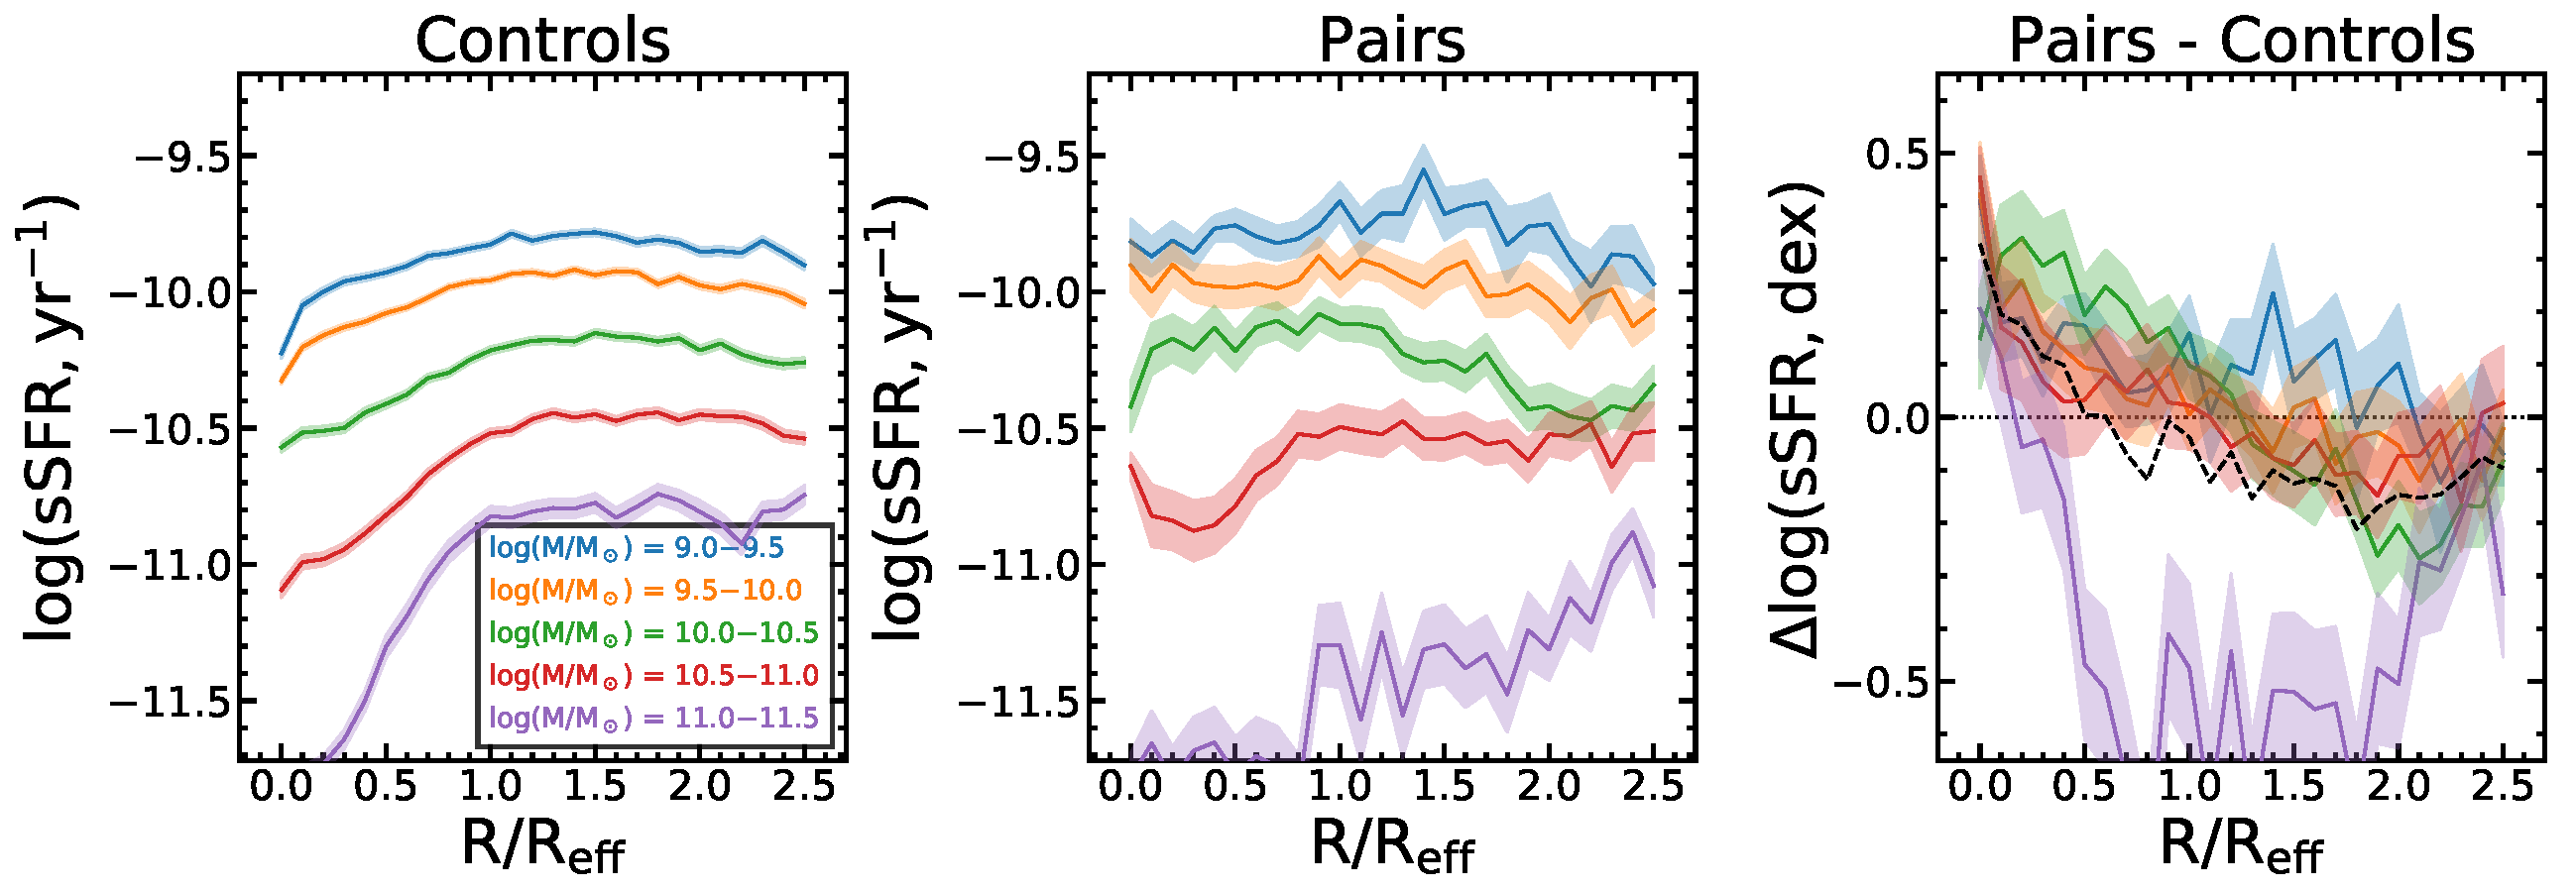
\includegraphics[width=\linewidth]{fig/ssfr_comb.pdf}
\caption[]{The log(sSFR) as a function of galactocentric radius for control galaxies (\textbf{Left}) and galaxy pairs (\textbf{Middle}). The difference between the profiles of the paired galaxies and the control galaxies are shown in the \textbf{Right} panel. The dashed black profile represents the mean of the difference profiles. The colors of the profiles represent the mass range of the selected galaxies which is given in the legend along with the number of galaxies in that mass bin in parantheses. The highlighted region around the profiles represent the standard error of the mean of the data at the given radius interval. The parts of the profiles with dashed lines represent regions where less than 50\% of the galaxies in the bin are covered at that radii. }
\label{fig:ssfr_prof}
\end{figure*}
%%%%%%%%%%%%%%%%%%%%%%%%%%%%%%%%%%%%%%%%%%%%%%

With the individual log(sSFR) profiles built for each MaNGA galaxy, we now use two different methods to compare the profiles of paired galaxies against the profiles of control galaxies. The first method, in Section \ref{sec:mass-bin}, paired galaxies are compared to control galaxies within evenly spaced stellar mass-bins. In the second method, in Section \ref{sec:tailored}, paired galaxies are compared to a subset of 20 control galaxies which are matched in stellar mass and redshift. 

\subsubsection{Mass-Binned Difference Profiles}\label{sec:mass-bin}

In the first method, paired and control galaxies are grouped into five evenly spaced stellar mass bins between \logm\ $=$ 9.0$-$11.5. Within each stellar mass bin, we create a median profile of log(sSFR) as a function of galactocentric radius for both paired and control galaxies. The control profiles are constructed using all available control galaxies within each mass bin. The error associated with the profile is the standard error of mean of the data at each radius bin. We show these ``stacked" profiles for control galaxies in the left hand panel of Figure \ref{fig:ssfr_prof} and the stacked profiles for paired galaxies in the middle panel of Figure \ref{fig:ssfr_prof}.

The radial extent of our profiles go out to 2.6 \reff; however,  67\% of the MaNGA sample is designed to cover only 1.5 \reff\ of the galaxy. Also, the MaNGA galaxies are not always centered on a spaxel center, so the 0$^{\rm th}$ spaxel may fall outside of the innermost radii bin. Because of these issues, the centers or the outskirts of the stacked profiles may only represent a small subset of the galaxies in that mass bin. To account for this, we ``trim" the stacked profiles where a radius bin contains data for less than 50\% of the total set of galaxies. We represent the trimmed regions in our figures with dashed lines. In Figure \ref{fig:ssfr_prof}, galaxies below \logm\ $\le$ 10.0 have their innermost radii bin trimmed due to insufficient coverage.

Once the stacked profiles are made, we take the difference between the stacked profiles of the paired galaxies and the control galaxies, pair - control, in log space (this means that the difference profiles really represent a ratio between the pairs and controls in linear space). This gives us difference profile, $\Delta$log(sSFR), which shows us where the sSFR is enhanced or suppressed (shown in the right hand panel of Figure \ref{fig:ssfr_prof}). 

The control galaxies are quenched in their centers with respect to their disks and the difference between the sSFR in their centers and their disks increases with higher stellar masses (which was previously seen in the MaNGA survey in \citet{Belfiore:2018}). The paired galaxies show flattened star formation profiles where the level of the sSFR remains roughly consistent across their disks except for paired galaxies with stellar masses above \logm\ $=$ 10.5 which still show some central quenching. 

When taking the difference between the pairs and controls, the paired profiles are centrally enhanced by $\sim$0.35 $\pm$ 0.1 dex which then falls to zero around 1.2 \reff. In the outskirts of the pairs beyond 1.2 \reff, the pairs feature lightly suppressed sSFR of 0.0$-$0.1 dex. All of the mass ranges except for the highest mass range, \logm\ $=$ 11.0$-$11.5, trend closely to the median profile. For the most massive galaxies, \logm\ $=$ 11.0$-$11.5, the enhancement to the sSFR within 0.5 \reff\ is higher than the median profile at 0.5$-$0.6 dex. The sSFR enhancement in the sample seems to be mass independent except for the most massive galaxies which feature higher levels of sSFR enhancement.

It is also relevant to note that the driving factor behind the central enhancement to the sSFR in the difference profiles is really the quenching in the centers of the controls. While the mechanism for the quenching in galaxies is in dispute, the merger process seems to be capable of rejuvenating star formation in the centers of these galaxies resulting in the flatter sSFR profiles seen in the paired galaxies. Further, since the sSFR enhancement in the difference profiles is largely driven by the quenched controls, it may be more appropriate to describe isolated galaxies as being centrally quenched in comparison to paired galaxies or that the profiles of paired galaxies are flattened in their centers with respect to their controls. 

The higher rate of star formation within interacting galaxies will mean that the stellar mass in the interacting galaxies will grow at a faster rate compared to secular mass growth. The fractional mass growth rate is simply the difference between the sSFR profiles of the paired and control galaxies in linear space (pairs - controls) multiplied by a given timescale. We chose a timescale of 0.4 Gyr which is estimated to be the average timescale for the merger induced starburst \citep{Feng:2019}. 

Since the $\Delta$log(sSFR) is independent of galaxy mass, the fractional mass change will depend on the stellar mass of the paired galaxy. That is, since the amount of new stellar mass from merger induced interactions is roughly constant across galaxies of different stellar masses, lower mass galaxies will experience a greater change to their total stellar mass. Low mass galaxies, \logm\ $=$ 9.0$-$9.5, experience a fractional mass change of $\Delta M_{\rm merger}$/$M_{\rm total}$ $=$ 0.03 (3\%) while massive galaxies, \logm\ $=$ 11.0$-$11.5, experience a fractional mass change of $\Delta M_{\rm merger}$/$M_{\rm total}$ $=$ 0.001 (0.1\%). This shows that the merger induced mass growth is greatest in low mass galaxies. Further, the merger induced mass growth is restricted to the centers of the paired galaxies which will result in galaxies which have more prominent bulges in their centers. 

This mass-binning method has the benefit of a high S/N control profile since each mass bin will have hundreds of control galaxies while the median control profiles of the second method will only have 20 controls. On the other hand, this method only controls for a single galaxy parameter, stellar mass, though it is still relevant that the central enhancement of the sSFR in pairs is able to be observed. The profiles can also only be studied as a function of stellar mass so we are unable to study the profiles as a function of projected separation or mass ratio. 

%%%%%%%%%%%%%%%%%%%%%%%%%%%%%%%%%%%%%%%%%%%%%%
\begin{figure*}
\centering
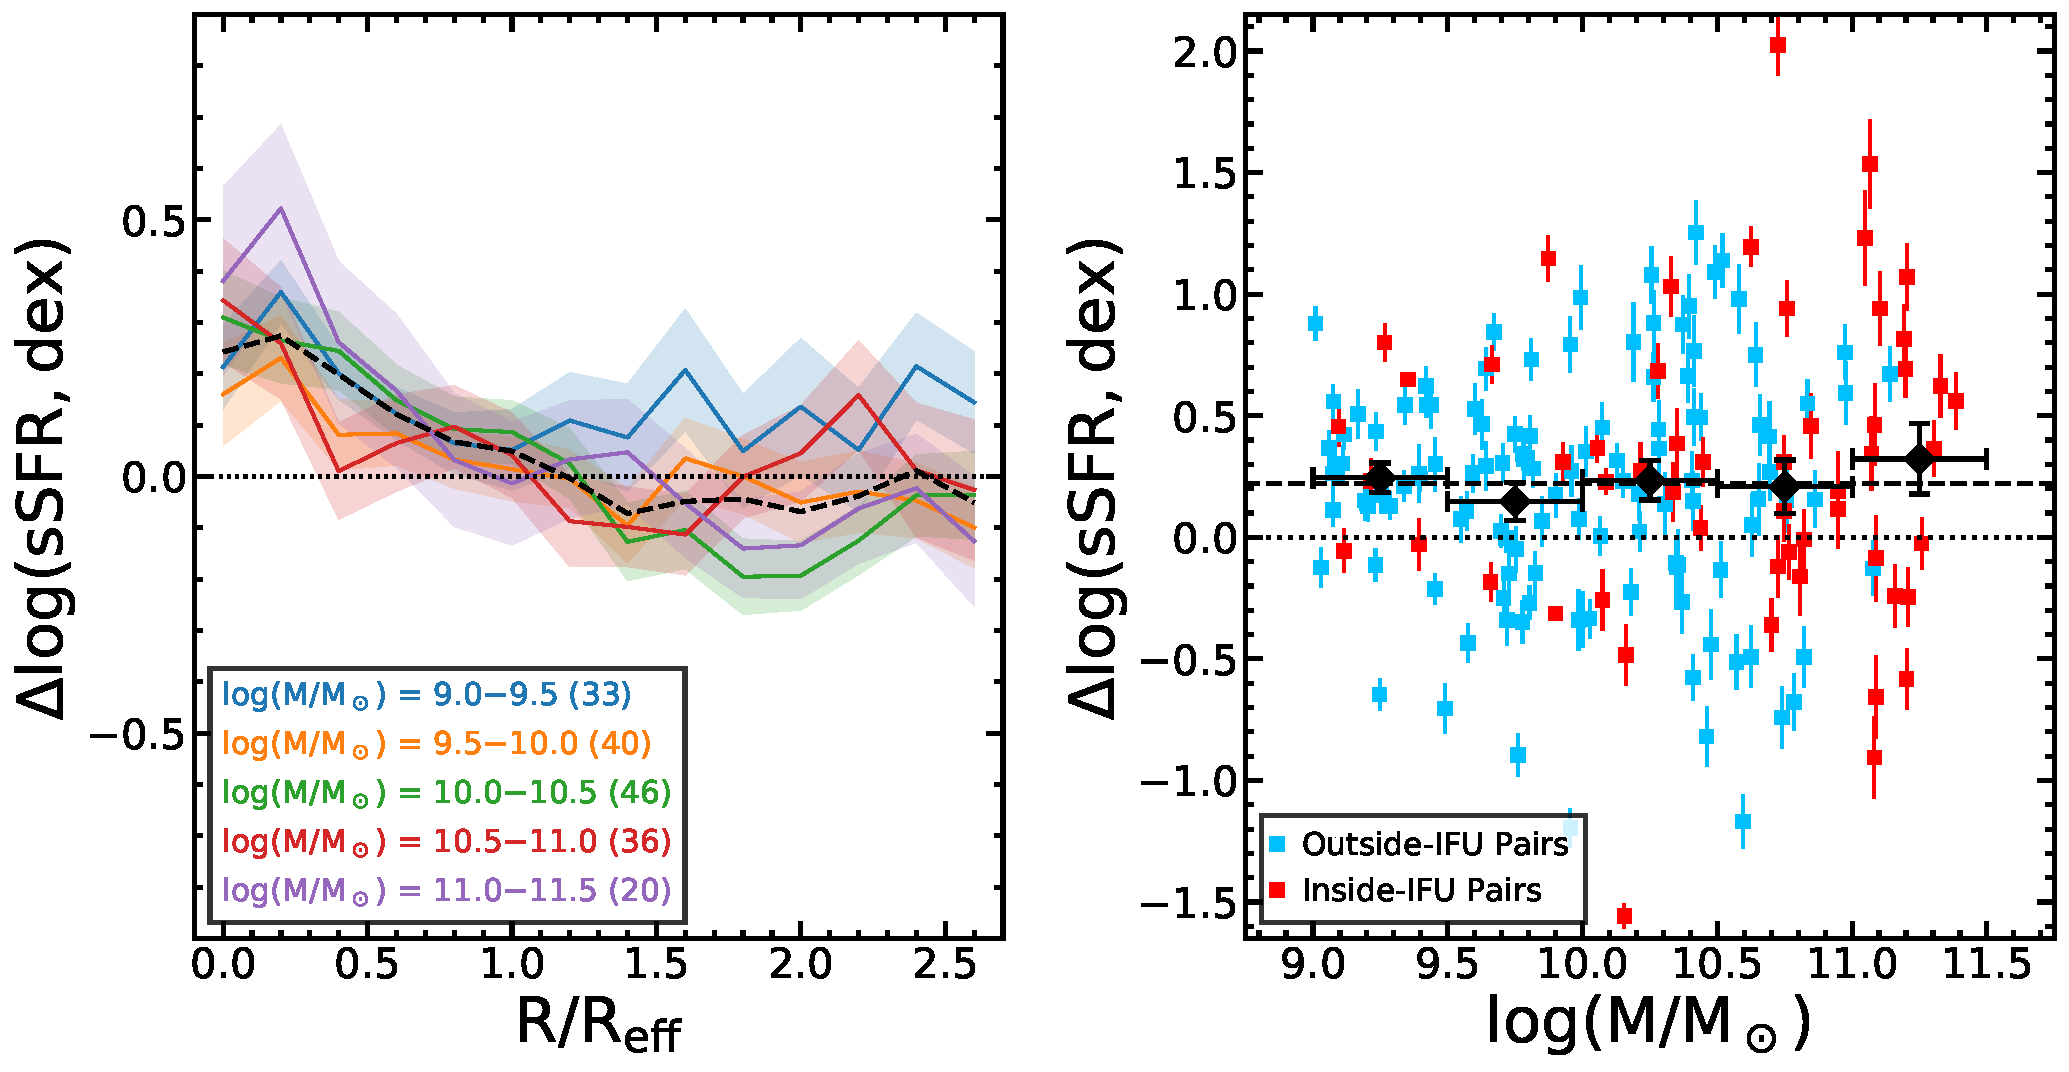
\includegraphics[width=\linewidth]{fig/ssfr_mass.pdf}
\caption[]{The \textbf{Left} panel shows the $\Delta$log(sSFR) profiles where the difference profiles are constructed from the difference between the paired galaxy profiles and a set of 20 control galaxies. The profiles are split into five different stellar mass bins and the highlighted region about the profiles represent the standard error of mean of the profile. The black dashed line represents the mean profile between the four difference mass ranges. The number of paired galaxies in each mass range is given in the legend in parentheses. In the \textbf{Right} panel the nuclear $\Delta$log(sSFR) are shown. The black squares are the mean values within a stellar mass bin (where the size of the bins are shown the the horizontal error bars). The vertical error bars on the black squares represent the standard deviation within the bin. The horizontal, dashed black line represents the median central enhancement of the pair sample. Galaxies in the outside-IFU (Blue) and inside-IFU (Red) samples are separately depicted.}
\label{fig:ssfr_mass}
\end{figure*}
%%%%%%%%%%%%%%%%%%%%%%%%%%%%%%%%%%%%%%%%%%%%%%

%%%%%%%%%%%%%%%%%%%%%%%%%%%%%%%%%%%%%%%%%%%%%%
\begin{figure}
\centering
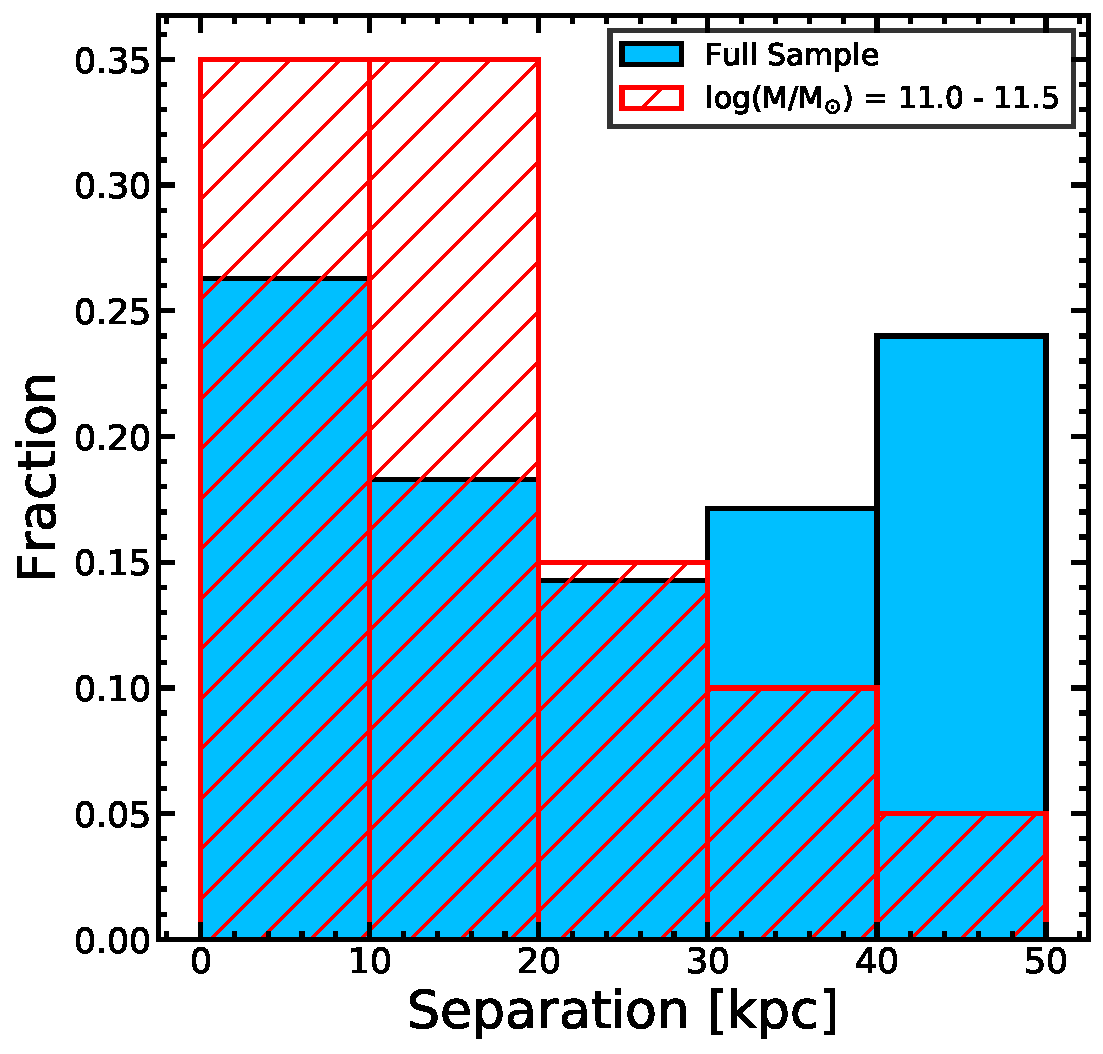
\includegraphics[width=\linewidth]{fig/sep_hist.pdf}
\caption[]{The projected separation distribution of the whole sample (blue) against the projected separation distribution for the highest mass galaxies, \logm\ $=$ 11.0$-$11.5 (Red). }
\label{fig:sep_hist}
\end{figure}
%%%%%%%%%%%%%%%%%%%%%%%%%%%%%%%%%%%%%%%%%%%%%%

\subsubsection{Tailored-Controls Difference Profiles}\label{sec:tailored}
%%%%%%%%%%%%%%%%%%%%%%%%%%%%%%%%%%%%%%%%%%%%%%
\begin{figure*}
\centering
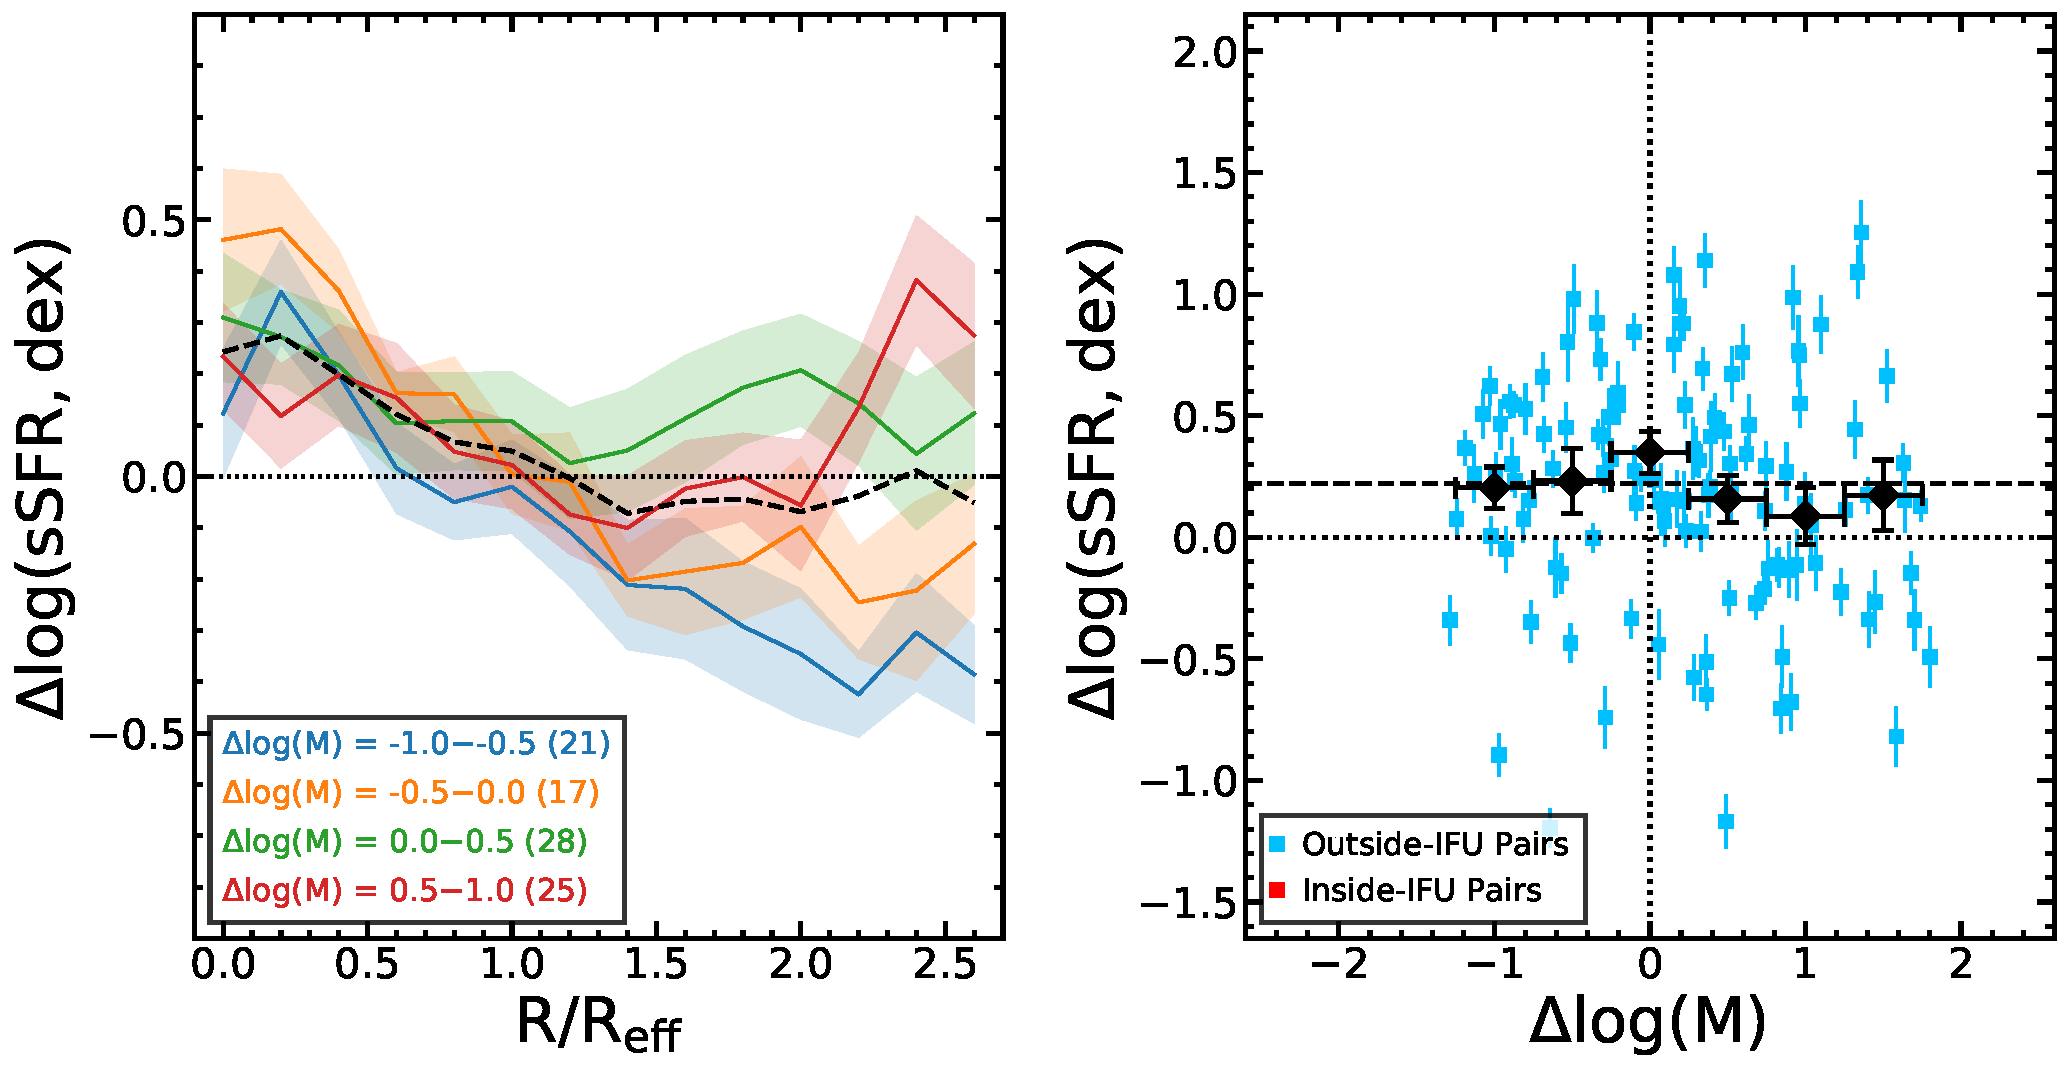
\includegraphics[width=\linewidth]{fig/ssfr_dm.pdf}
\caption[]{Same as Figure \ref{fig:ssfr_mass} except the difference profiles are split by mass ratio. The inside-IFU sample is left out of this analysis as their mass ratios are unreliable.}
\label{fig:ssfr_dm}
\end{figure*}
%%%%%%%%%%%%%%%%%%%%%%%%%%%%%%%%%%%%%%%%%%%%%%
In the second method, we match each paired galaxy to a set of 20 control galaxies of similar stellar masses and redshifts, as described in Section \ref{sec:control}. We take the individual azimuthally averaged profiles of the selected control galaxies and take the median value of the profiles at each radius bin to produce the median profile of the control galaxies. 

Once the median profile of the control galaxies is made, we take the difference between the paired galaxy's profile and the median control profile in log space. We do this process for each of the 175 paired galaxies. 

The difference profiles at this stage have now been controlled for both stellar mass and redshift. We can freely stack these difference profiles to study their dependence on other parameter like the mass ratio and projected separation. 

First, we split the profiles by stellar mass to see how this method compares to the previous mass-binning method. We split the individual difference profiles into five evenly spaced stellar mass bins between \logm\ $=$ 9.0$-$11.5 and stack the difference profiles within each mass bin. This gives us five difference profiles covering five different stellar mass ranges shown in the left hand panel of Figure \ref{fig:ssfr_mass}. The errors of the stacked profiles are the standard error of the mean of the difference profiles within each bin.

To focus on the sSFR offsets in the centers of the galaxies, we take the median sSFR within 0.5 \reff\ for all galaxies. We then calculate the offsets in the centers of the pairs by taking the difference between the sSFR in the centers of the pairs and the median sSFR of their 20 controls. We depict the central $\Delta$log(sSFR) as a function of stellar mass in the right hand panel of Figure \ref{fig:ssfr_mass}

The difference profiles are shown to be centrally enhanced by $\sim$0.25 $\pm$ 0.1 dex. Similar to what was seen in Section \ref{sec:mass-bin}, the level of the enhancement is independent of galaxy mass with the exception of the highest mass bin, \logm\ $=$ 11.0$-$11.5, which is 0.15$-$0.25 dex higher than the sample average. 

The central enhancement to the sSFR falls to zero around 1.2 \reff\ and the outskirts of the galaxies are lightly suppressed by 0.1 dex. The paired galaxies in the mass range, \logm\ $=$ 9.0$-$9.5, feature enhanced sSFR in their disks of 0.1$-$0.2 dex. As we will show in the next section, Section \ref{sec:dm}, the offsets seen in the disks of paired galaxies are largely driven by whether the galaxy is the more massive or less massive companion in the pair.

To understand why these high mass galaxies behave differently from the rest of the sample, we compare the distribution of the projected separation for the whole sample and for galaxies in the highest mass bin in Figure \ref{fig:sep_hist}. The whole sample has a v-shaped separation distribution. This is the result of the combination of the two different samples, the inside-IFU and outside-IFU samples. The outside-IFU sample should find more pairs at wide projected separations due to the larger volume to find companions in. The separation distribution of the inside-IFU sample is limited by MaNGA's IFU sizes and the sample's redshift distribution; the maximum possible projected separation for a MaNGA target with $z$ $=$ 0.15 and a 127 spaxel IFU is about 40 kpc. The highest mass galaxies in the sample are at closer projected separations in comparison to the rest of the sample with 70\% of the highest mass galaxies being within 20 kpc. As we will show in Section \ref{sec:sep}, the central sSFR enhancement is strongest at small projected separation which means that higher sSFR in the centers of the massive galaxies may be driven by their close projected separations. 

The results we obtain from the tailored-control method is largely consistent with the mass-binning method. Between the two methods we see that the $\Delta$log(sSFR) profile is independent of the total stellar mass of the galaxies. In the next two sections, we will use the tailored-control method to study how the profiles behave as a function of the mass ratio (Section \ref{sec:dm}) and projected separation (Section \ref{sec:sep}).

\subsection{Dependency on Mass Ratio}\label{sec:dm}

%%%%%%%%%%%%%%%%%%%%%%%%%%%%%%%%%%%%%%%%%%%%%%
\begin{figure*}
\centering
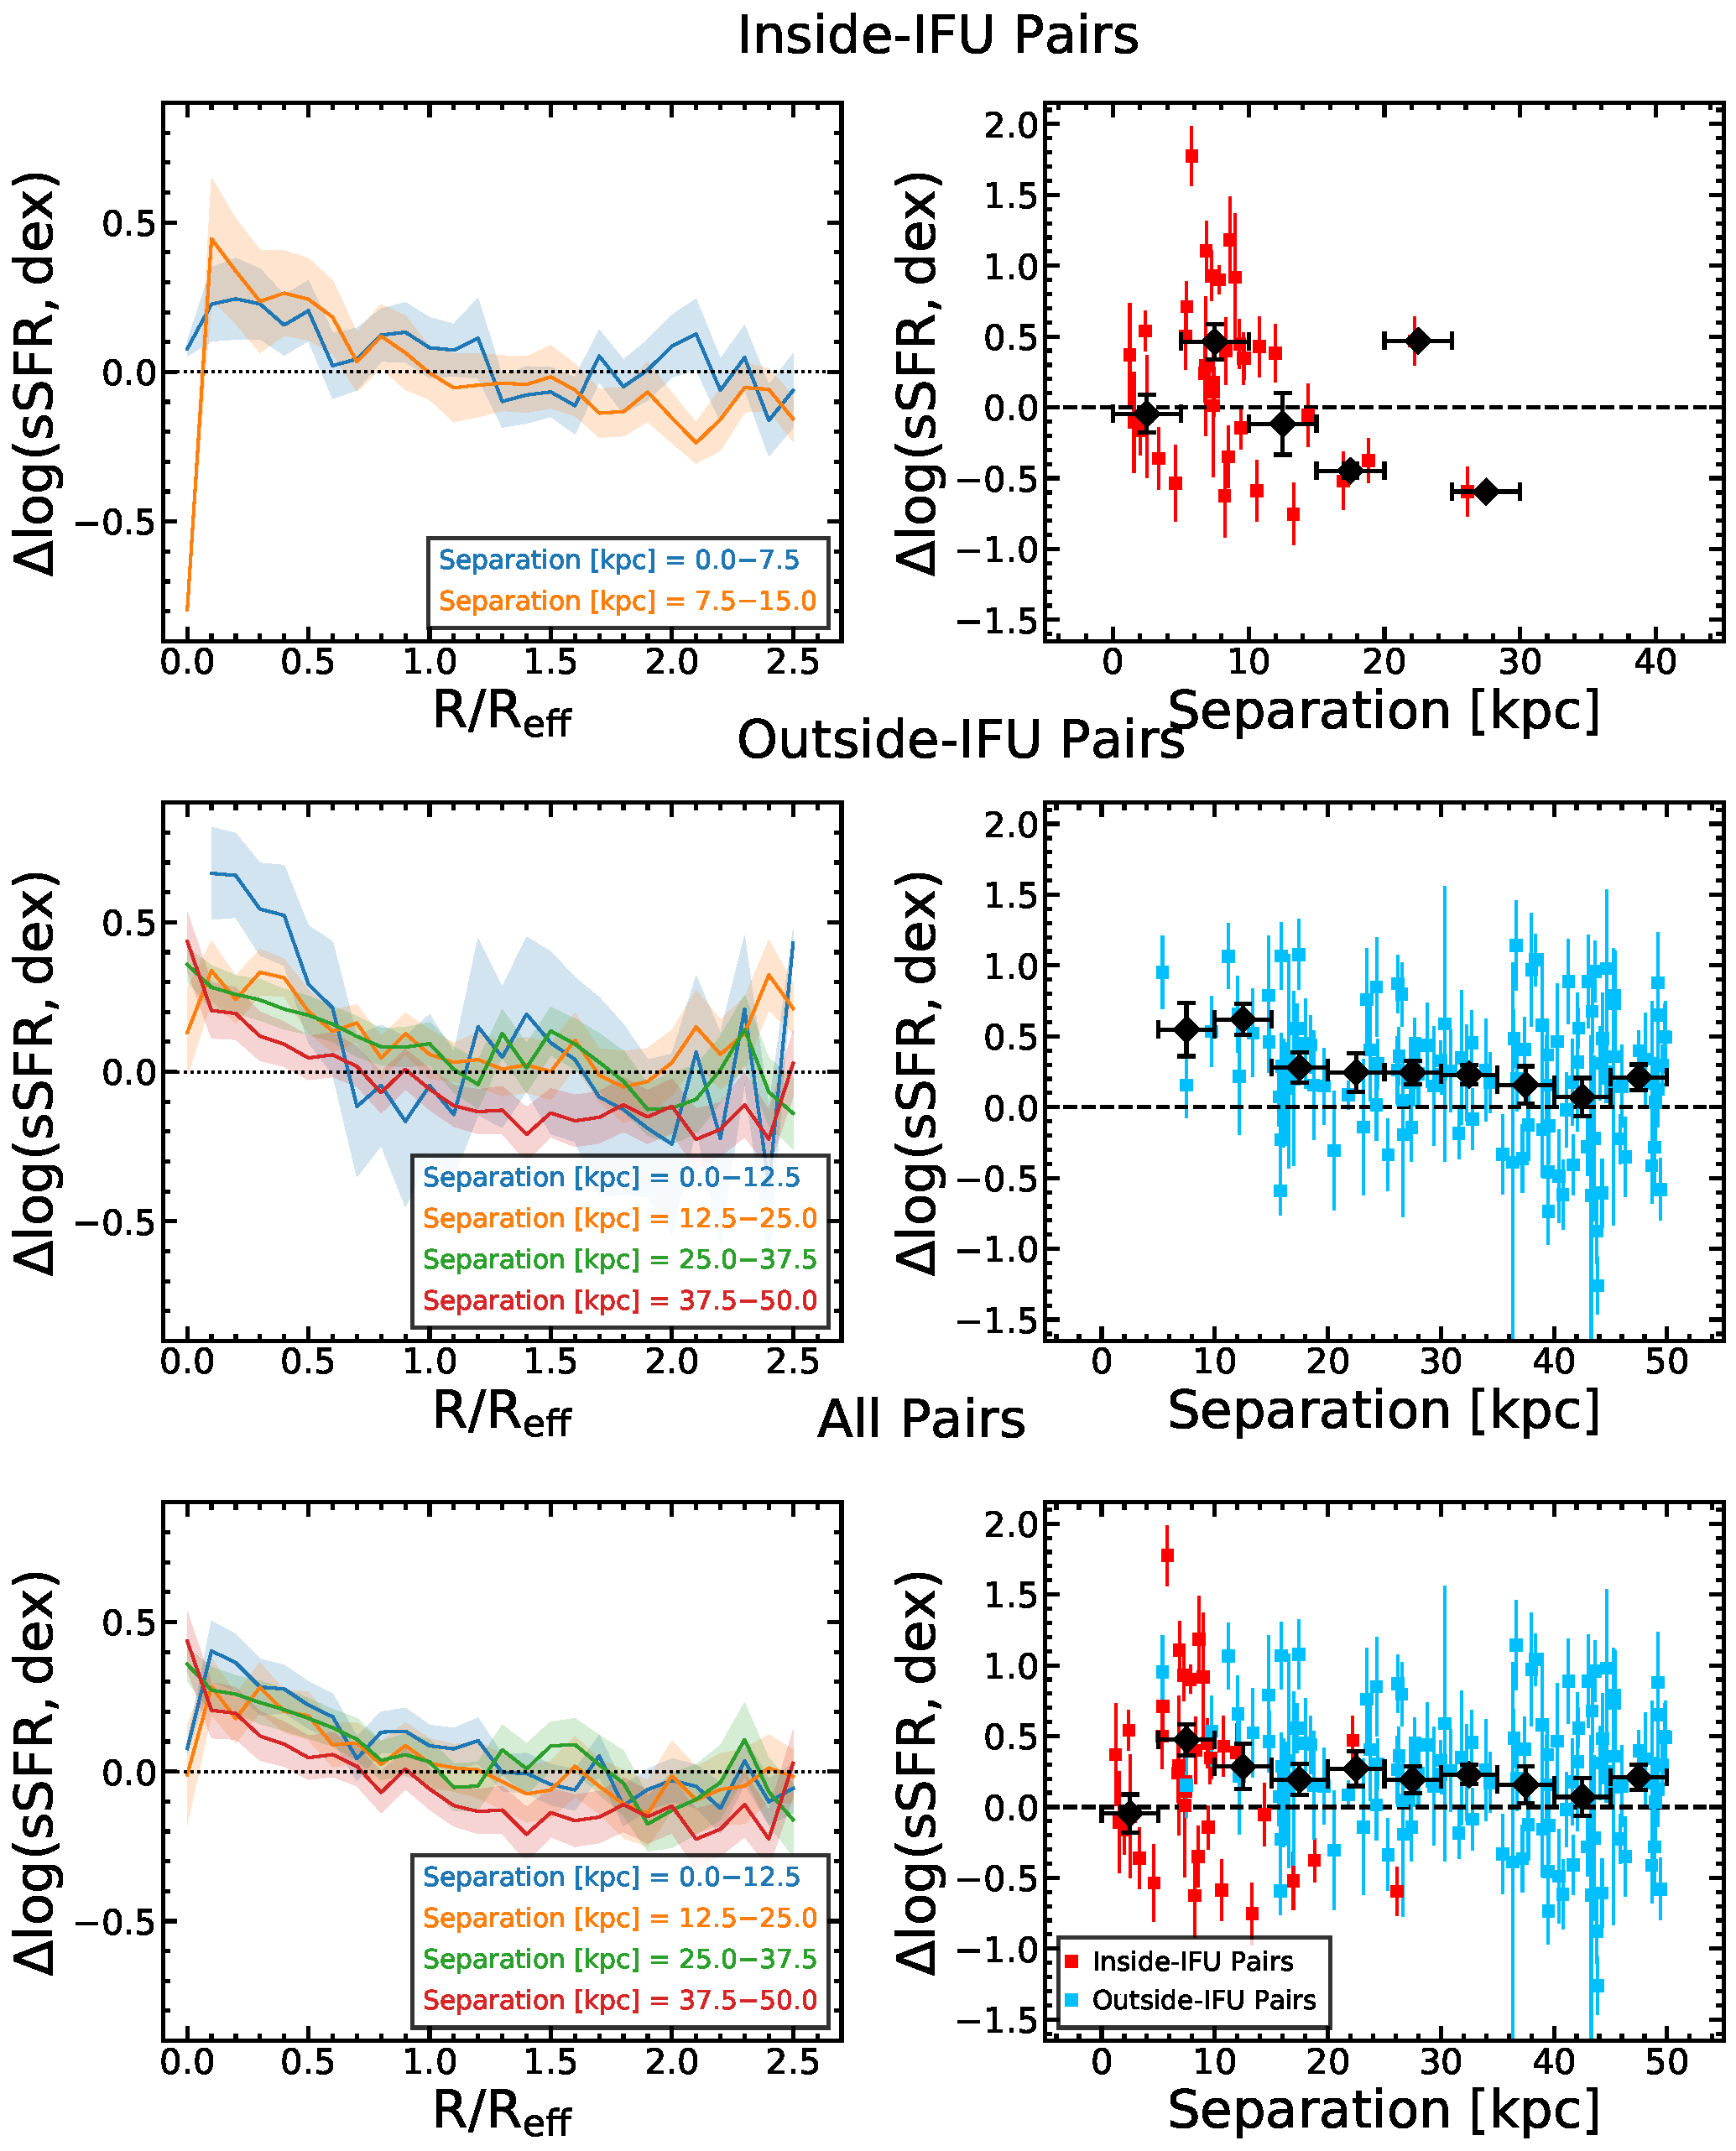
\includegraphics[width=\linewidth]{fig/ssfr_sep.pdf}
\caption[]{Same as Figure \ref{fig:ssfr_mass} except the difference profiles are split by projected separation. }
\label{fig:ssfr_sep}
\end{figure*}
%%%%%%%%%%%%%%%%%%%%%%%%%%%%%%%%%%%%%%%%%%%%%%



While the total stellar mass of the galaxies has no effect on the merger induced star formation, the mass ratio between the paired galaxies does. The mass ratio here is calculated as the difference between stellar masses contained within the 50\% half light radius, 

\begin{equation}
\Delta {\rm log}(M) = {\rm log}(M_{\rm target}) - {\rm log}(M_{\rm comp}) 
\end{equation}

Where $M_{\rm target}$ is the stellar mass of the MaNGA target galaxy and $M_{\rm comp}$ is the stellar mass of the companion galaxy. We will define the more massive galaxies of a pair, $\Delta$log($M$) $>$ 0.0, the primary companion and the less massive galaxy of a pair, $\Delta$log($M$) $<$ 0.0, the secondary companion.

For the outside-IFU sample we use the stellar masses calculated from the $r$-band elliptical Petrosian apertures from the NSA catalog. Most of the companion galaxies in the inside-IFU sample are not covered by either the NSA catalog or \citet{Simard:2011}. Because of this, the inside-IFU galaxies are left out of this analysis.

In the top left of Figure \ref{fig:ssfr_dm}, we split the profiles by mass ratio in four bins; the primary and secondary companion of a major merger, $|\Delta$log($M$)$|$ $<$ 0.5, and the primary and secondary companion of a minor merger, $|\Delta$log($M$)$|$ $>$ 0.5. Regardless of the mass ratio, the centers of the paired galaxies are centrally enhanced, though major mergers have stronger enhancements in their centers by $\sim$0.2 dex over minor mergers. Secondary companions also feature slightly higher levels of enhancement in their centers than primary companions at the same mass ratios by $\sim$0.1 dex. 

The sSFR offsets in the outskirts of the galaxy pairs show a dependence on the mass ratio. Primary companions show a zero to positive enhancement of 0.0$-$0.4 dex to the sSFR in their outskirts. Secondary companions feature a suppression to the sSFR in their outskirts of about 0.1$-$0.4 dex. 

In the top right of Figure \ref{fig:ssfr_dm} we see that the sSFR enhancement is strongest in galaxies close to a 1:1 mass ratio, $\Delta$log($M$) $=$ 0.0. These galaxies feature a central enhancement of $\sim$0.35 dex which is 0.1 dex higher than the average central enhancement of the whole sample. This enhancement falls with wider mass ratio; however, pairs with large differences in stellar mass still feature substantial levels of star formation enhancement, 0.15$-$0.20 dex at mass ratios of $|\Delta$log($M$)$|$ $=$ 1.0. We also see that secondary companions show a higher level of sSFR enhancement, by $\sim$0.1 dex, with respect to primary companions. 

%To emphasize the difference between primary and secondary companions and to further investigate the sSFR enhancement seen in the outskirts of low mass galaxies (\logm\ $=$ 9.0$-$9.5), we plot the difference profiles split both by stellar mass and mass ratio in Figure \ref{fig:ssfr_massdm}. The difference profile of primary companions is centrally enhanced by 0.25 dex and remains enhanced across their disks with an enhancement of 0.1-0.3 dex. The difference profile of secondary companions is centrally enhanced by 0.3 dex and is suppressed by 0.1 dex in their outskirts. Specifically looking at the paired galaxies in the mass range, \logm\ $=$ 9.0$-$9.5, the primary companions in the mass range show strong enhancements to their outskirts while the primary companions in the mass range show a weak suppression to their outskirts. 

From the mass ratio, we see two different effects. First, we see that the central enhancement to the sSFR is strongest for pairs with 1:1 mass ratios. Second, we see that secondary companions show steeper enhancement profiles with higher levels of sSFR enhancement in their centers and stronger levels of sSFR suppression in their disks with respect to primary companions. It is interesting to note that the central enhancement to sSFR is dependent on both the mass ratio and the projected separation (which we will demonstrate in the next section) while the sSFR offsets in their outskirts primarily depends on whether the galaxy is the primary or secondary companion of the pair.

\subsection{Dependency on Projected Separation}\label{sec:sep}

We look at the level of sSFR enhancement as a function of the projected separation between the two galaxies in Figure \ref{fig:ssfr_sep}. The $\Delta$log(sSFR) profiles show a clear gradient with the projected separation with close galaxy pairs showing higher levels of sSFR enhancement compared to pairs with wide separations. The profiles in the galaxy pairs in the separation range, $r_{\rm p}$ $=$ 0.0$-$12.5, are generally $\sim$0.05$-$0.1 dex above the median and the profiles of the galaxy pairs in the separation range, $r_{\rm p}$ $=$ 37.5$-$50.0, are generally $\sim$0.05$-$0.1 dex below the median. 

This effect can be seen more clearly in the scatter plot of the central $\Delta$log(sSFR) enhancement as a function of projected separation. The level of the enhancement gradually increases with closer separation from 50 kpc to 10 kpc. While $\Delta$log(sSFR) falls at higher separations, there is still a substantial level of enhancement between 40 and 50 kpc, $\sim$0.1$-$0.2 dex. Within 20 kpc, the $\Delta$log(sSFR) enhancement jumps to 0.3$-$0.4 dex. 

The sSFR enhancement increasing with closer projected separations is to be expected and has been shown in previous studies \citep{Li:2008, Ellison:2008, Scudder:2012, Patton:2013}. The passage of the first pericenter is predicted to trigger a burst of star formation which falls as the two galaxies separate \citep{Scudder:2012}. The sSFR enhancement in our sample persists out to 50 kpc and previous works have shown that the burst of star formation can persist out to 150 kpc \citep{Patton:2013}. 



%%%%%%%%%%%%%%%%%%%%%%%%%%%%%%%%%%%%%%%%%%%%%%%%%%%%
\section{Discussion}\label{sec:disc}

%Among the three parameters, stellar mass, mass ratio, and projected separation, the projected separation has the strongest effect on the $\Delta$log(sSFR) enhancement, followed by the mass ratio. From this we see that the paired galaxies with the strongest enhancements to the central sSFR are paired galaxies with 1:1 mass ratios and  which are within 10 kpc. 

%Between the splitting the $\Delta$log(sSFR) profile by stellar mass, mass ratio, and projected separation, we see that the general shape of the profile within the inner 1.0 \reff\ is unchanged. The profile is peaked in the center of the paired galaxies and linearly (in log space) to zero around 1.0 \reff. Different projected separations and mass ratios may elevate or suppress the level of the enhancement in the profile's center; however, the shape of the profile is largely unchanged.

\subsection{Comparison with Previous Works}

%%%%%%%%%%%%%%%%%%%%%%%%%%%%%%%%%%%%%%%%%%%%%%
\begin{figure}
\centering
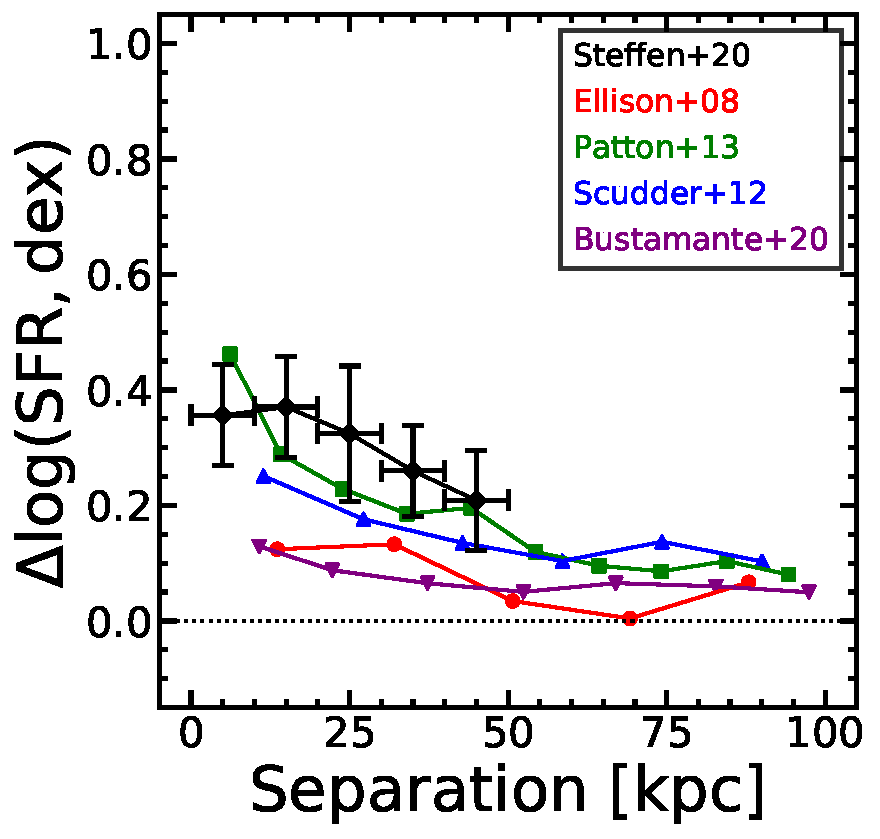
\includegraphics[width=3in]{fig/nuc_sep.pdf}
\caption[]{(\textbf{Top}) $\Delta$log(SFR) over projected separation for this sample using the tailored control method (Black), \citet{Ellison:2008} (Red),  \citet{Scudder:2012} (Blue), \citet{Patton:2013} (Green), and \citet{Bustamante:2020} (Purple). (\textbf{Bottom}) $\Delta$log(sSFR) over projected separation for this sample (Black), \citet{Li:2008} (Red), and \citet{Patton:2020} (Blue).  }
\label{fig:nuc_sep}
\end{figure}
%%%%%%%%%%%%%%%%%%%%%%%%%%%%%%%%%%%%%%%%%%%%%%

The $\Delta$log(SFR) as a function of projected separation has been studied before with the SDSS survey \citep{Ellison:2008, Li:2008, Patton:2013, Scudder:2012, Bustamante:2020}. We compare the mentioned surveys with our own work in Figure \ref{fig:nuc_sep}. We find that our central SFR enhancements for closely separated pairs are higher than many of the previous studies, our sSFR enhancement is $\sim$0.2 dex higher than \citet{Scudder:2012} and $\sim$0.3 dex higher than \citet{Ellison:2008} and \citet{Bustamante:2020}. The central enhancement to the sSFR for closely separated pairs in our sample is $\sim$0.1 dex higher than \citet{Patton:2013}. The sSFR enhancement function from \citet{Li:2008} follows closely to our own and remains $\sim$0.05 dex above our sample out to 40 kpc.  

The sSFR as a function of separation was studied with the cosmological hydrodynamical simulations of IllustrisTNG \citep{Patton:2020}. In Figure \ref{fig:nuc_sep} we show the $\Delta$log(sSFR) enhancements across 2D separation (projected separation) from the TNG300-1 simulation. \citet{Patton:2020} found a sSFR enhancement which is 1.8$\times$ that of the isolated controls within a separation of 15 kpc and is statistically significant out to a 2d separation of $\sim$250 kpc. This enhancement is $\sim$0.1 dex lower than ours; however, our sSFR enhancement shown in Figure \ref{fig:nuc_sep} was extracted from a 0.5 \reff\ aperture while \citet{Patton:2020} extracted the sSFR from a 50\% half-mass radius. This means that our extraction radius is effectively twice a small and is more restricted to the central burst of star formation. 

Our sample only covers projected separations within 50 kpc, while previous surveys cover out to 100$-$200 kpc. While our sample covers a smaller separation range, the $\Delta$log(SFR) of our sample at 50 kpc is roughly the same level as \citet{Scudder:2012} and \citet{Patton:2013} at the same projected separation. From this we see that our sSFR enhancement as a function of projected separation is consistent with with what has been found in previous works. 

\citet{Li:2008} studied the star formation enhancement over different stellar masses and saw that low mass galaxies experience greater levels of enhancement than high mass galaxies.  Galaxies in the mass range \logm\ $=$ 9.72 were shown to experience an enhancement $\sim$0.4 dex higher than galaxies in the mass range \logm\ $=$ 10.6. In this work, we find that $\Delta$log(sSFR) has no dependence on the stellar mass of the galaxy. The source of the difference is unclear; between our works we utilize different methods for determining the sSFR enhancement in galaxy pairs. \citet{Li:2008} defines their enhancement function as the average sSFR of the paired galaxies at a given separation, weighted by the number of companions, subtracted by the average sSFR of the whole sample. While we don't find the same dependency between the sSFR enhancement and stellar mass, the sSFR enhancement as a function of projected separation between our studies is in good agreement.

The dependency of the SFR enhancement on the mass ratio was studied in \citet{Ellison:2008}. They found that pairs with mass ratios of 2:1 have higher SFR enhancements of $\sim$0.1 dex over pairs with wider 10:1 mass ratios. We find that pairs with mass ratios of $\Delta$log($M$) $=$ 0.25 (1.8:1) are 0.2 dex over pairs with mass ratios of $\Delta$log($M$) $=$ 1.0 (10:1). \citet{Ellison:2008} also saw tentative evidence for SFR enhancement in the secondary companions of minor pairs. We not only confirm that secondary companions of minor pairs feature SFR enhancement, but also that the enhancement is higher than the primary component of pairs at the same mass ratios. 

In Figure \ref{fig:prof_comp} we compare the $\Delta$log(sSFR) profile as a function of galactocentric radius between our work and previous works. The post-merger galaxies in \citet{Thorp:2019} have sSFR enhancements between $\sim$0.05$-$0.2 dex higher than our sample of paired galaxies. The centers of the post-merger galaxies feature a greater level of sSFR enhancement in their centers compared to our galaxies pairs of $\Delta$log(sSFR) $=$ 0.5, roughly 0.25 dex higher than our paired galaxies. The post-merger galaxies also feature enhanced sSFR in their disk past 1.0 \reff\ of $\sim$0.1$-$0.15 dex. The heightened level of sSFR enhancement in the centers of post-merger galaxies in comparison to merging galaxies seems consistent with the idea that a second and greater burst of star formation occurs as the two merging galaxies coalesce into a single galaxy. 

The galaxy pairs in \citet{Pan:2019} have sSFR enhancements that are roughly $\sim$0.1$-$0.2 dex higher than our sample. Our paired galaxies show a slight sSFR suppression in their disks past 1.0 \reff\ while the galaxy pairs in \citet{Pan:2019} show an enhancement of $\sim$0.15 dex to the sSFR in their disks. The reason for the discrepancies between our samples may be that \citet{Pan:2019} includes a set of post-merger galaxies while our sample has no post-merger galaxies. These post-merger galaxies are predicted to have higher levels of star formation over other paired galaxies due to a second larger burst of star formation which is triggered as the merging galaxies coalesce and may be able to increase the sample's average sSFR enhancement . 

\citet{Barrera-Ballesteros:2015} studied the sSFR in paired galaxies in the CALIFA IFS survey using the H$\alpha$ equivalent width (\ewha) as a proxy for the sSFR. They compared the sSFR in the centers of paired galaxies to their disks by varying the aperture diameters from which they extract the \ewha. They found that the sSFR is enhanced in the centers of the paired galaxies but suppressed in their disks, which is similar to what we find.  

\citet{Moreno:2015} used {\sc Gadget}-3, a smoothed particle hydrodynamics code, to study the spatial extent of the star formation enhancement. The merger simulations showed that the star formation enhancement was largely concentrated in the centers (R $<$ 1 kpc) of the paired galaxies and that the off-nuclear regions (1 $<$ R $<$ 10 kpc) showed a suppression to the star formation. \citet{Moreno:2015} also found that lower mass secondary galaxies (in mergers with stellar mass ratios of 2.5:1) have higher levels of sSFR enhancement in their centers and have stronger levels of sSFR suppression in their disks. This is in good agreement with our work, we found that secondary companions show moderately higher levels of sSFR enhancement in their centers in comparison to primary companions at the same mass ratio. Further, the outskirts of the primary companions feature positive to zero enhancement to their sSFR while the secondary companions show a strong suppression to the sSFR in their outskirts. 

%%%%%%%%%%%%%%%%%%%%%%%%%%%%%%%%%%%%%%%%%%%%%%%%%%%%
\section{Summary and Conclusion}\label{sec:sum}

%%%%%%%%%%%%%%%%%%%%%%%%%%%%%%%%%%%%%%%%%%%%%%
\begin{figure}
\centering
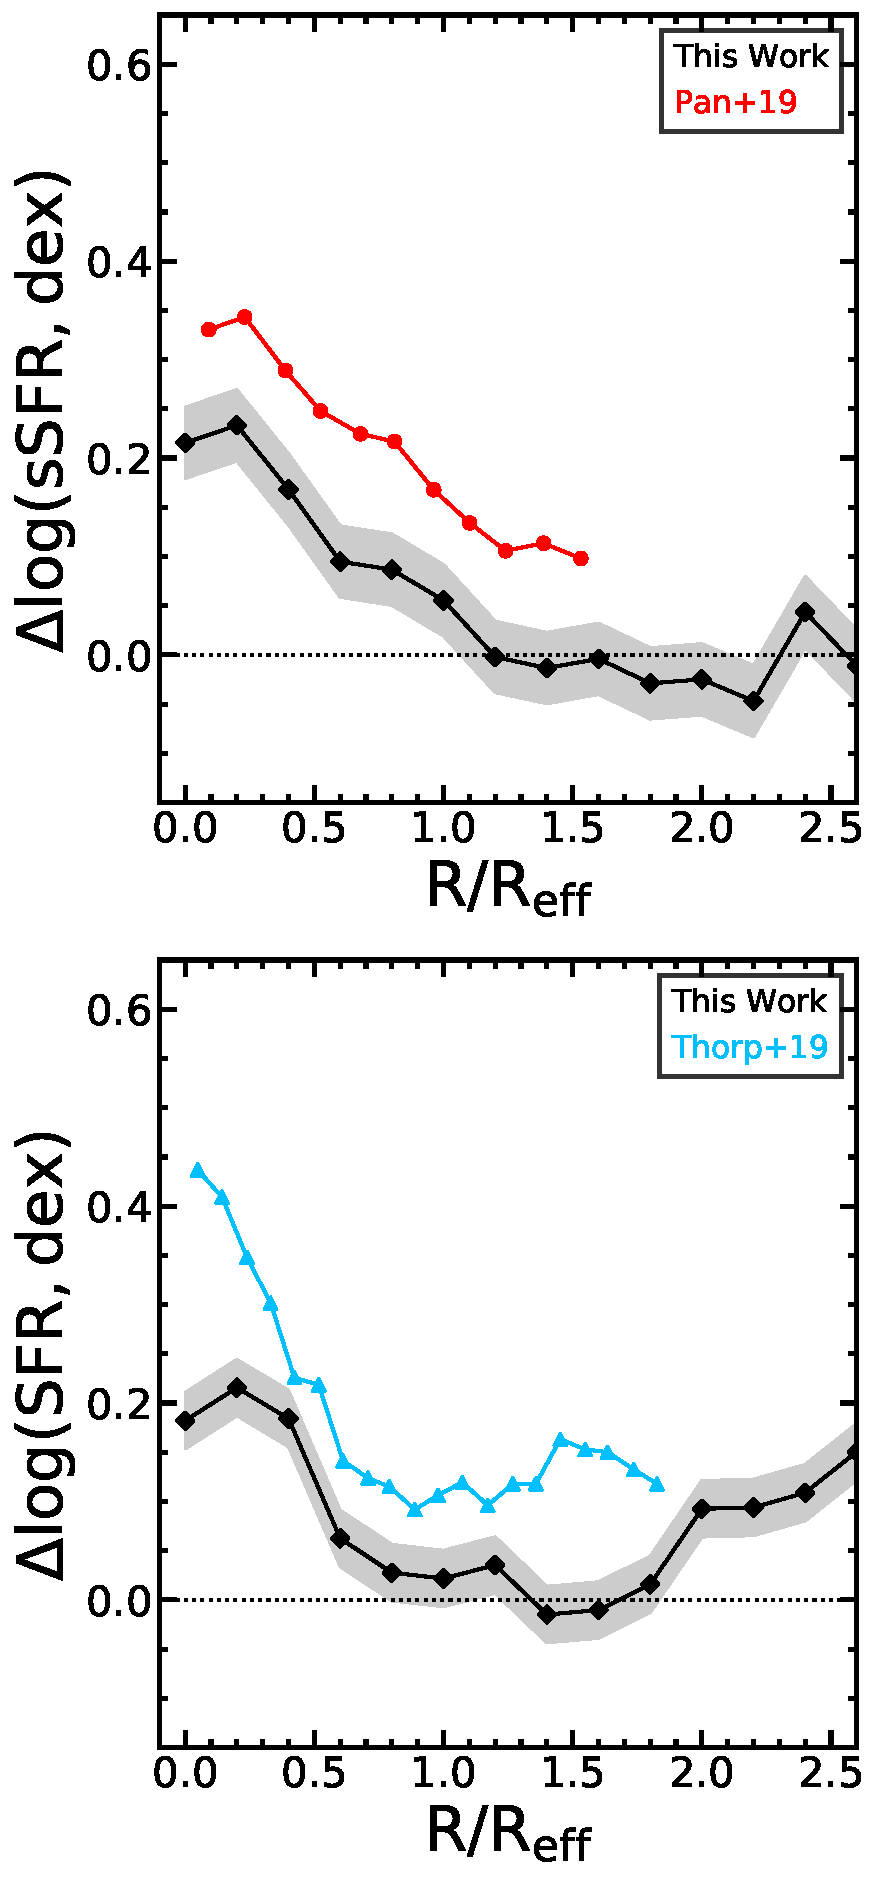
\includegraphics[width=3in]{fig/prof_comp.pdf}
\caption[]{The mean radial profile of $\Delta$log(sSFR) between pairs and controls of this work with the tailored control method (Black) compared against those of \citet{Pan:2019} (Red) and \citet{Thorp:2019} (Blue).}
\label{fig:prof_comp}
\end{figure}
%%%%%%%%%%%%%%%%%%%%%%%%%%%%%%%%%%%%%%%%%%%%%%

In this work. we have made a sample of 175 star forming galaxy pairs along with a set of 1888 star forming control galaxies in the MaNGA IFS survey. We compared the radial profiles of sSFR between the paired galaxies and controls galaxies and found the following;

\begin{enumerate}
\item The sSFR is centrally enhanced within the inner 1.0 \reff\ by 0.25 $\pm$ 0.1 dex. 
\item The outskirts of the paired galaxies, \reff\ $=$ 1.0$-$2.5, show limited suppression in their disks of $\sim$0.1 dex.
\item The sSFR enhancement in paired galaxies is independent of their total stellar mass.
\item The sSFR enhancement in paired galaxies does depend on the ratio between the masses of the paired galaxies. Galaxies with small mass ratios, $|\Delta$log($M$)$|$ $=$ 0.0$-$0.5, see an enhancement to sSFR of 0.35 dex, which is 0.1 dex higher than the average paired galaxies in the survey. Paired galaxies with large mass ratios, $|\Delta$log($M$)$|$ $=$ 1.0, still show substantial levels of enhancement to the sSFR, 0.1$-$0.2 dex. 
\item The secondary companions of a galaxy pair, the less massive galaxy, show higher sSFR enhancements, by $\sim$0.1 dex in comparison to primary companions at the same mass ratio. Further, primary companions have zero to positive sSFR offsets in their ouskirts, $\Delta$log(sSFR) $=$ 0.0$-$0.4 dex. Secondary companions feature a sSFR suppression in their outskirts of 0.1$-$0.4 dex.
\item The sSFR enhancement increases with closer projected separations where galaxies within 20 kpc have their sSFR enhanced by 0.3$-$0.4. 
\end{enumerate}

There is still much to be understood about these galaxy pairs. We see that there is a great diversity in the difference profiles of individual galaxies. In particular there are galaxy pairs which feature a strong suppression to the sSFR in their centers while others feature a central enhancement to the sSFR which is much greater than the median enhancement. The depth of our analysis here would benefit by studying other merger parameters like the interaction stage or the gas fraction. 

As of August 24, 2020, MaNGA has finished observing its goal of 10,000 galaxies. The completion of the final sample will mean that we will have access to a larger sample of paired and control galaxies. We also plan to fit the light profiles of the inside-IFU companion galaxies which will allow us to roughly double the size of the inside-IFU sample. With this and the completion of MaNGA's observations, we may be able to expand our pair sample to include nearly 500 galaxy pairs.

With the larger sample size we will be better able to separate how the stellar mass, mass ratio, and projected separation effect the enhancement profile along with new parameters like the merger stage and gas fraction. Also, by constructing enhancement profiles for the inside-IFU companions to the MaNGA targets, we can better study how primary companions behave in comparison to their secondary companions. 

\acknowledgments

% funding
We thank Cheng Li for our useful discussion on how the sSFR enhancement in galaxy pairs relates to their stellar mass and mass ratio. J.S. and H.F. acknowledge support from the National Science Foundation (NSF) grant AST-1614326. Funding for the Sloan Digital Sky Survey IV has been provided by the Alfred P. Sloan Foundation, the U.S. Department of Energy Office of Science, and the Participating Institutions. SDSS acknowledges support and resources from the Center for High-Performance Computing at the University of Utah. The SDSS web site is www.sdss.org.

SDSS is managed by the Astrophysical Research Consortium for the Participating Institutions of the SDSS Collaboration including the Brazilian Participation Group, the Carnegie Institution for Science, Carnegie Mellon University, the Chilean Participation Group, the French Participation Group, Harvard-Smithsonian Center for Astrophysics, Instituto de Astrofísica de Canarias, The Johns Hopkins University, Kavli Institute for the Physics and Mathematics of the Universe (IPMU) / University of Tokyo, the Korean Participation Group, Lawrence Berkeley National Laboratory, Leibniz Institut für Astrophysik Potsdam (AIP), Max-Planck-Institut für Astronomie (MPIA Heidelberg), Max-Planck-Institut für Astrophysik (MPA Garching), Max-Planck-Institut für Extraterrestrische Physik (MPE), National Astronomical Observatories of China, New Mexico State University, New York University, University of Notre Dame, Observatório Nacional / MCTI, The Ohio State University, Pennsylvania State University, Shanghai Astronomical Observatory, United Kingdom Participation Group, Universidad Nacional Autónoma de México, University of Arizona, University of Colorado Boulder, University of Oxford, University of Portsmouth, University of Utah, University of Virginia, University of Washington, University of Wisconsin, Vanderbilt University, and Yale University.

%%%%%%%%%%%%%%%%%%%% REFERENCES %%%%%%%%%%%%%%%%%%
\bibliographystyle{aasjournal}
\bibliography{mergerbib}

\end{document}